\chapter[Modelos de seleção de características]{Modelos de seleção de características}

\section{Modelos de Seleção de Características}

Como visto, existem várias maneiras e técnicas para se montar um modelo para seleção de características, podendo-se combinar as formas de busca, e as várias maneiras de avaliar os subconjuntos gerados, e os critérios de parada para chegar a um modelo que seja adequado ao problema, ou seja, encontrando um subconjunto que sejá otimizado em relação ao conjunto inicial. A combinação das técnicas geram três possíveis categorias de modelos: o modelo de filtro (\textit {filter}), o modelo de envelopamento (\textit {wrapper}) e o modelo híbrido (\textit {hybrid}). 

\subsection{Modelo de Filtro (\textit{filter})}

Os algoritmos de filtro não necessitam de um algoritmo de \textit{machine learning} para poder fazer a seleção de características, utilizando-se somente das próprias características para poder avaliar os subconjuntos, geralmente necessitando de um menor poder computacional para poder serem utilizados. A Figura 4 ilustra como trabalha um algoritmo de filtro.

\begin{figure}[h]
	\centering
	\label{fig05}
		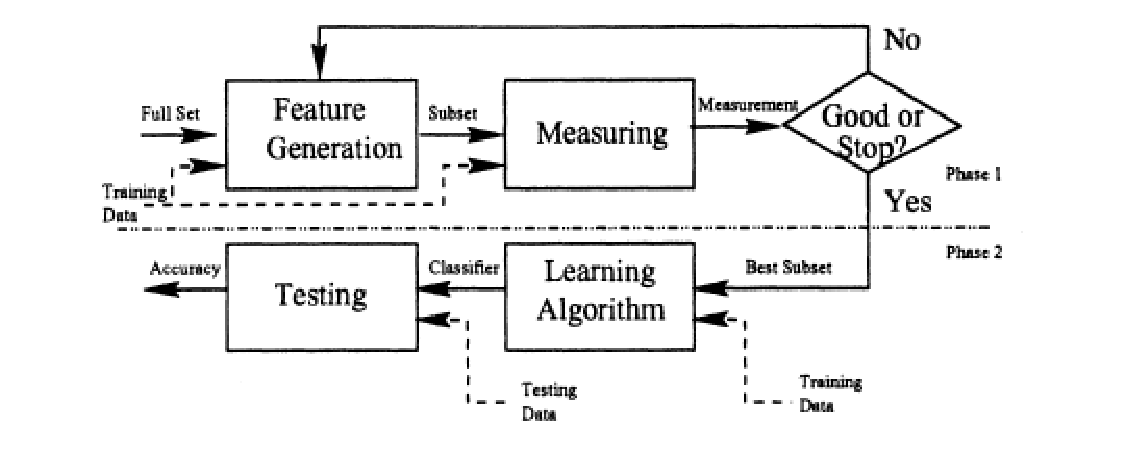
\includegraphics[keepaspectratio=true,scale=1]{figuras/fig05.eps}
	\caption{Fluxograma do modelo de filtro (\textit{filter}). \cite{huan_1998}}
\end{figure}

O modelo é composto por duas fases, a primeira fase consiste em selecionar o melhor subcojunto possível utilizando alguma das medidas citadas no capítulo anterior para poder avaliar esses subconjuntos. A segunda fase consiste em utilizar o subconjunto gerado em um classificador. Nessa fase também é colocado os dados de treino no classificador para avaliar se o resultado foi satisfatório. Os algoritmos de filtro não dependem da avaliação do classificador, e sim das informações e medidas obtidas diretamente dos dados. \cite{huan_1998}

Pode-se generalizar o modelo de filtro de acordo com a Figura 5, onde para um dado conjunto \textit{D} de características, é escolhido um subconjunto \textit{S0} através de alguma das formas de busca. Cada subconjunto gerado é avaliado e comparado com o seu anterior, sempre sendo escolhido aquele que tenha um melhor valor em seu critério de avaliação ($\gamma$). Esse processo será repetido até que um critério de parada ($\alpha$) seja alcançado ou que sejam testados todos os conjuntos possíveis. \cite{liu_2005}

\begin{figure}[h]
	\centering
	\label{fig06}
		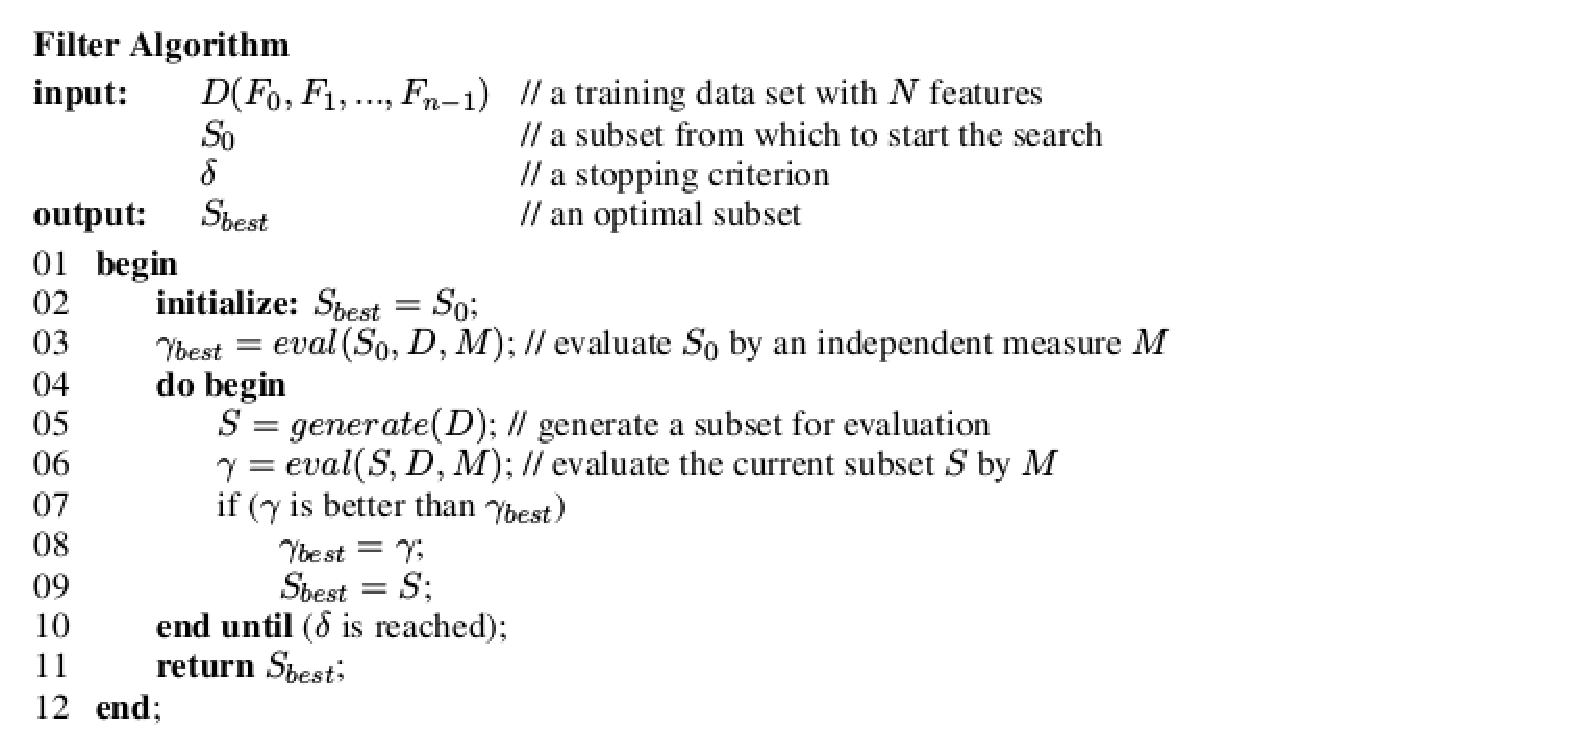
\includegraphics[keepaspectratio=true,scale=0.7]{figuras/fig07.eps}
	\caption{Generalização do algoritmo de filtro (\textit{filter}). \cite{liu_2005}}
\end{figure}

\subsection{Modelo de Envelopamento (\textit{wrapper})}

Os algoritmos que se baseiam no modelo de envelopamento necessitam de um algoritmo de \textit{machine learning} pré determinado para que seja possível utiliza-lo. Isso se deve ao fato de que o modelo usa o próprio classificador para avaliar o quão bom é o subconjunto de dados gerado, utilizando a acurácia do classificador para avaliar os subconjuntos. A Figura 6 ilustra como funciona um algoritmo de envelopamento.

\begin{figure}[h]
	\centering
	\label{fig07}
		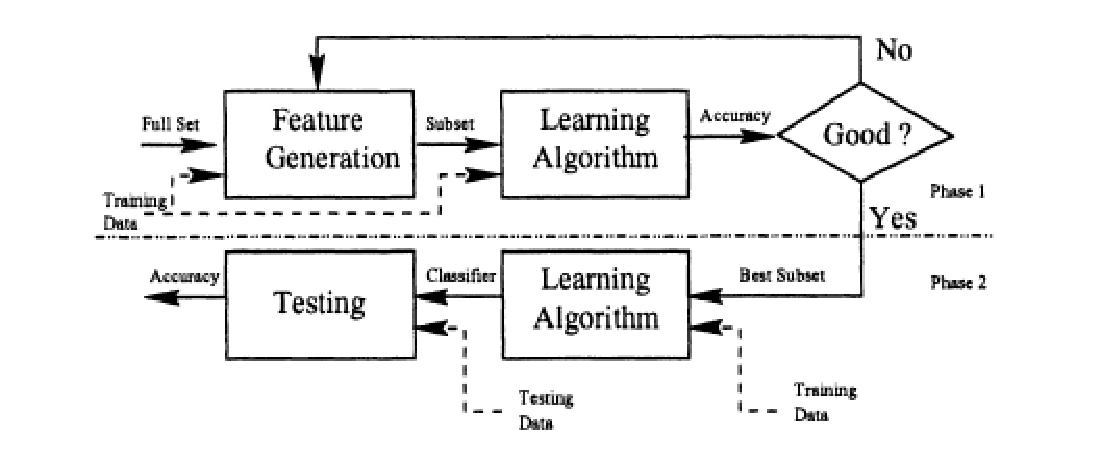
\includegraphics[keepaspectratio=true,scale=1]{figuras/fig06.eps}
	\caption{Fluxograma do modelo de envelopamento (\textit{wrapper}). \cite{huan_1998}}
\end{figure}

O modelo é composto por duas fases, a primeira fase consiste em escolher um subconjunto utilizando um classificador para poder avaliar o quão bom é esse subconjunto. Já a segunda fase é igual a do modelo de filtro, onde o subconjunto é utilizado no classificador e então são inseridos os dados de treino para verificar se o resultado foi realmente satisfatório.

Pode-se generalizar o modelo de envelopamento de acordo com a Figura 7, onde para um dado conjunto \textit{D} de características, é escolhido um subconjunto \textit{S0} através de alguma das formas de busca. Cada conjunto gerado é avaliado e comparado com o seu anterior utilizando um algoritmo de \textit{machine learning}, sempre sendo escolhido aquele que tenha um melhor valor em seu critério de avaliação ($\gamma$). Esse processo será repetido até que um critério de parada ($\alpha$) seja alcançado ou que sejam testados todos os conjuntos possíveis. \cite{liu_2005}


\begin{figure}[h]
	\centering
	\label{fig08}
		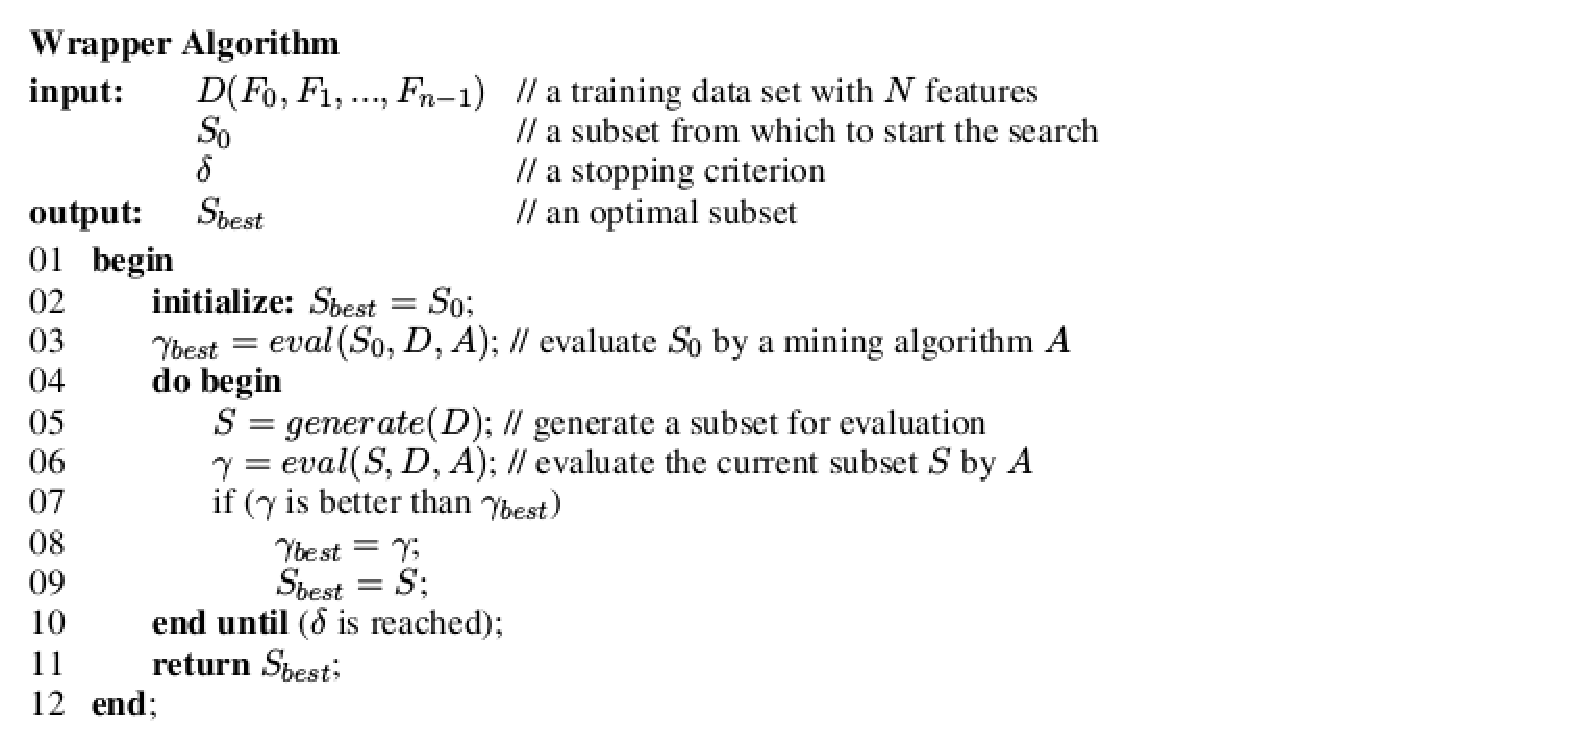
\includegraphics[keepaspectratio=true,scale=0.7]{figuras/fig08.eps}
	\caption{Generalização do algoritmo de envelopamento (\textit{wrapper}). \cite{liu_2005}}
\end{figure}

\subsection{Modelo Híbrido (\textit{hybrid})}

Os algoritmos que se baseiam no modelo híbrido são compostos por técnicas do modelo de filtro e de envelopamento. O modelo híbrido busca utilizar da melhor forma possível os dois modelos para poder alcançar um melhor subconjunto. Geralmente utiliza-se o modelo híbrido para problemas como muitos dados \cite{liu_2005}. Na Figura 8 veremos como seu algorítimo funciona.

\begin{figure}[h]
	\centering
	\label{fig09}
		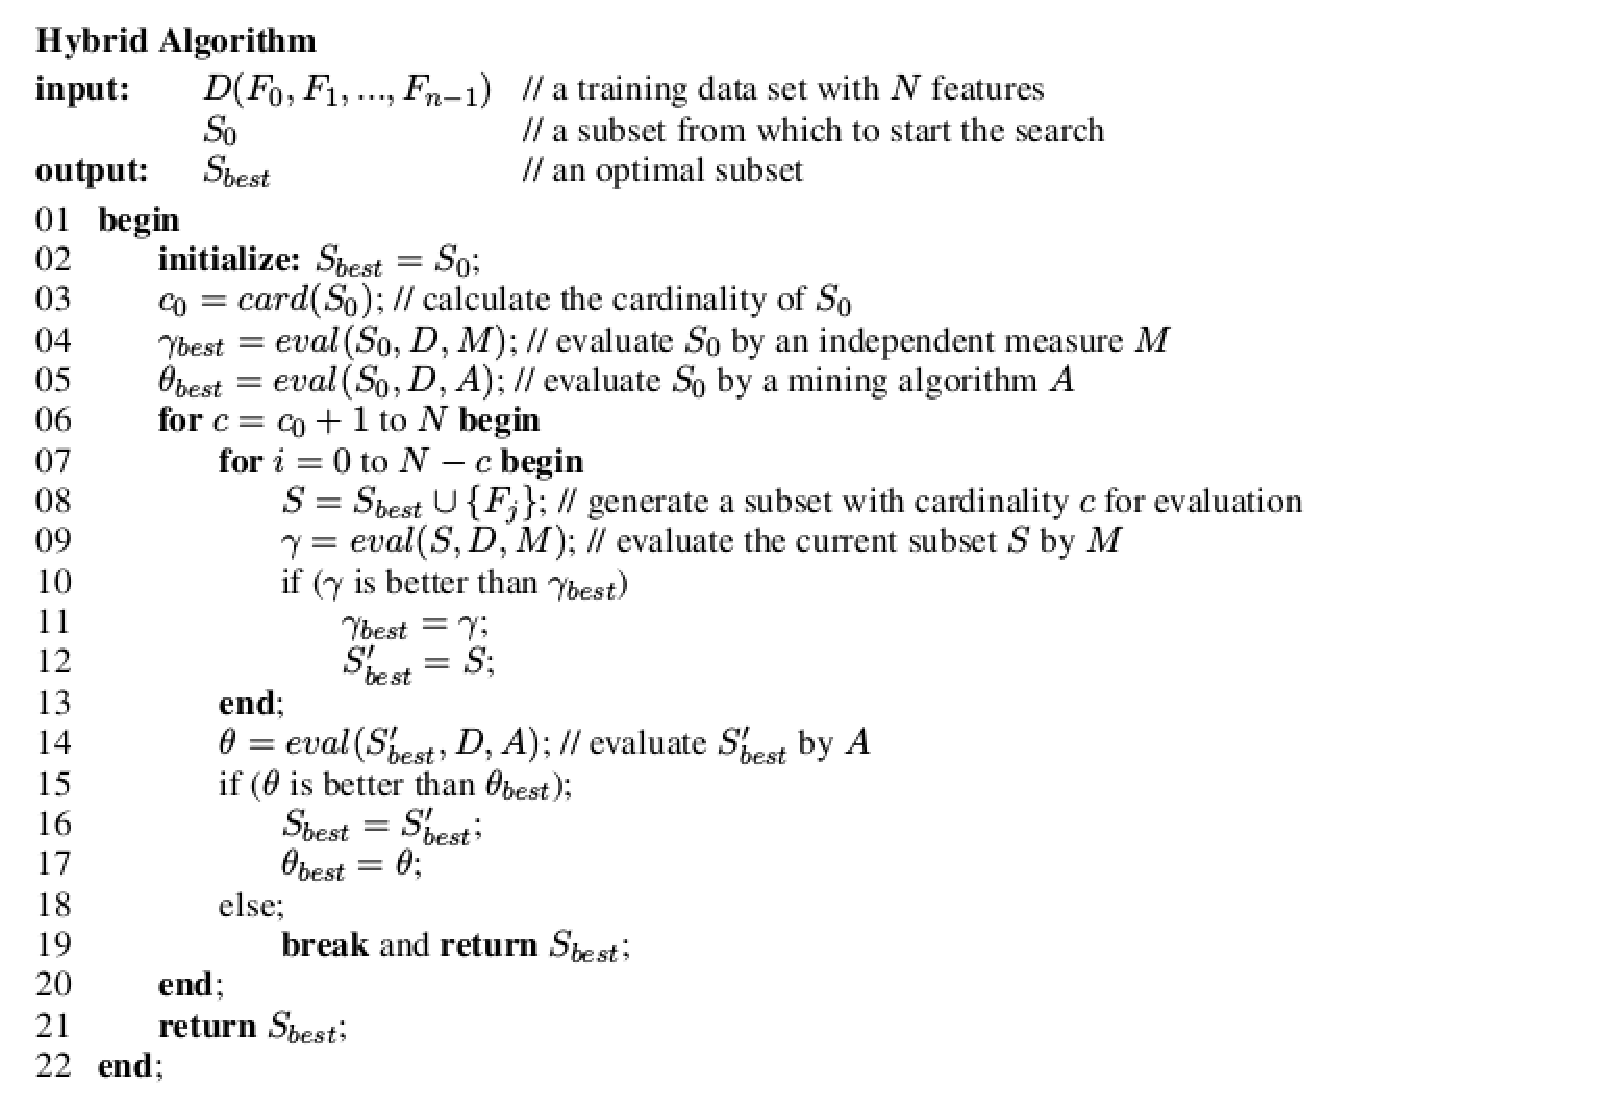
\includegraphics[keepaspectratio=true,scale=0.7]{figuras/fig09.eps}
	\caption{Generalização do algoritmo híbrido (\textit{hybrid}). \cite{liu_2005}}
\end{figure}

Para um dado conjunto \textit{D} de características, é escolhido um subconjunto \textit{S0} através de alguma das formas de busca, geralmente utiliza-se um conjunto vazio e é adicionado características a cada iteração. A cada iteração se adiciona uma característica e é comparada subconjunto a subconjunto dessa iteração utilizando medidas independentes ($\gamma$), ou seja, das características em si, que terá c + 1 características, até que seja possível encontrar o melhor subconjunto. Repete-se o processo até que se ache o melhor subconjunto de cada uma das iterações, e então esses subconjunto serão então comparados utilizando algum classificador ($\theta$), para que seja obtido o melhor subconjunto possível. \cite{liu_2005}

\section{Modelos Escolhidos}

\subsection{\textit{Relief-F} - Modelo de Filtro}

Esse modelo foi escolhido pelo fato de ser muito utilizado e obter bons resultados, como apontado por \citeonline{dash_1997} e \citeonline{liu_2005}. O maior problema encontrado com o algoritmo foi o fato de seu predecessor, o Relief, tratar apenas de classes binárias, o que traria certos problemas quanto a escolha das bases de dados a serem utilizadas no trabalho, assim como problemas quanto a compatibilidade de bases que seriam submetidas ao serviço que esse trabalho se propõe a implementar. \textit{Relief-F} resolve esse impasse quanto ao tipo das bases de dados.

O algoritimo \textit{Relief-F} utiliza métodos estatísticos para selecionar as características relevantes, é um método que se baseia nos pesos atribuídos às caracterísicas \cite{dash_1997}. O algorítmo realiza a busca de maneira sequêncial e utiliza medidas de distância para poder realizar a avaliação entre as características. Primeiramente o algorítmo inicializa os pesos (\textit{W}) com 0, e escolhe um valor de limite ($\phi$), então para uma característica \textit{n} ele calcula os valores de \textit{Near Hit} e \textit{Near Miss}, ambos calculados através da distância euclidiana. \textit{Near Hit} é a menor distância entre instancias de mesma classe, já o \textit{Near Miss} é o menor valor entre instancias de classes diferentes. Depois de percorrer todas as características ele retorna aquelas que têm o valor do peso maior do que o limite estabelecido. Esse processo está representado na Figura 9.

\begin{figure}[h]
	\centering
	\label{fig11}
		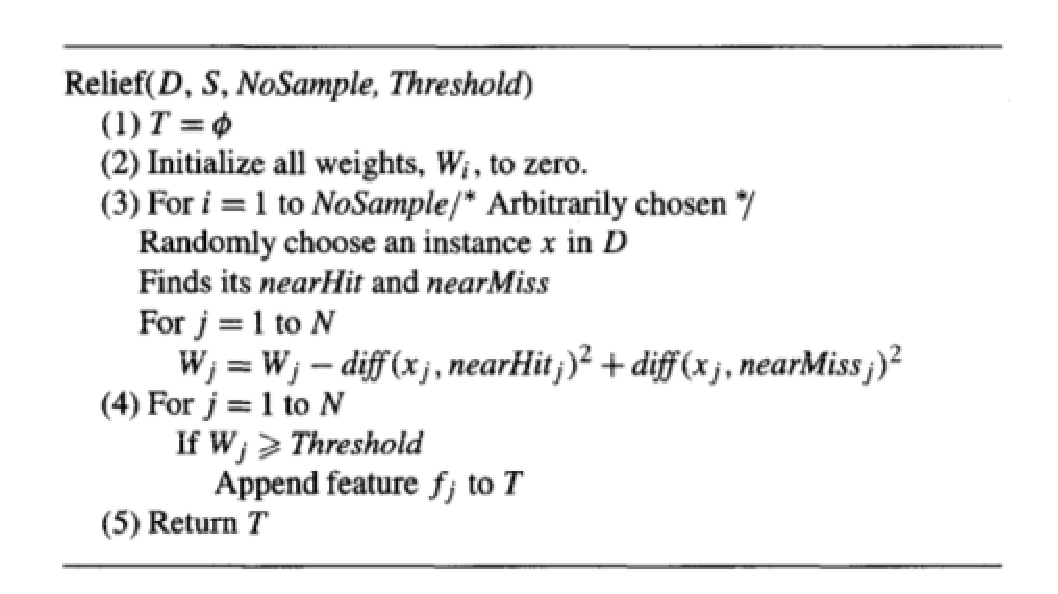
\includegraphics[keepaspectratio=true,scale=0.7]{figuras/fig11.eps}
	\caption{Representação do Modelo Relief-F. \cite{dash_1997}}
\end{figure}

\subsection{Método da Árvore de Decisão - \textit{Decision Tree Method (DTM)} - Modelo de Filtro}

O modelo DTM foi escolhido por ser um modelo de funcionamento um tanto peculiar, uma vez que se utiliza o algoritmo C4.5 para realizar a seleção de características, ou seja, utiliza-se um classificador para poder escolher as características, porém ele não é um algorítmo de seleção de Envelopamento (\textit{wrapper}), ele continua sendo um algorítmo do tipo Filtro (\textit{filter}) pelo fato de utilizar medidas internas do classificador relacionadas a erro, e não só as medidas de acurácia. \cite{dash_1997}. Após montar a árvore de decisão, é feita a 'poda' da árvore, e é dessa árvore 'podada' que são extraídas as características que serão utilizadas no classificador final, não sendo necessário ser o C4.5. 

Na Figura 10 é visto como é proposto esse modelo. Pode parecer simples, porém o maior trabalho advém do algoritmo C4.5, que realizará todos os calculos e montará a árvore que servirá de insumo para o classificador final.

\begin{figure}[h]
	\centering
	\label{fig12}
		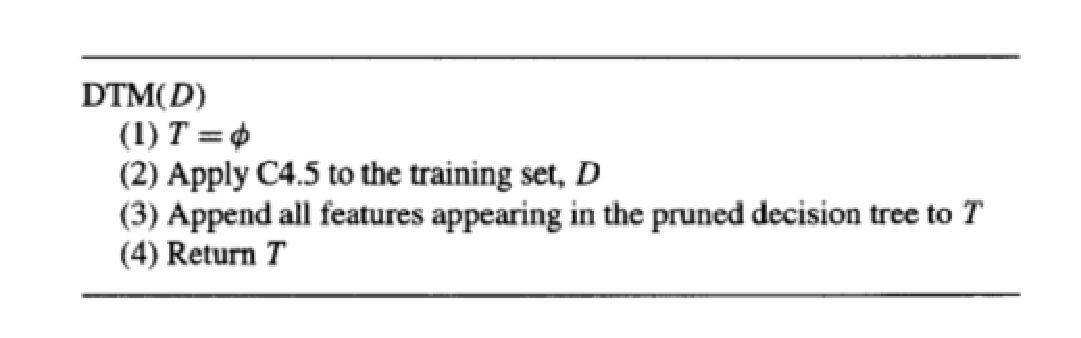
\includegraphics[keepaspectratio=true,scale=0.7]{figuras/fig12.eps}
	\caption{Representaçao do Modelo DTM. \cite{dash_1997}}
\end{figure}

\subsection{\textit{Linear Forward Selection (LFS)} - Modelo de Envelopamento}

A escolha do modelo LFS foi feita com base na premissa de que já haviam sido escolhidos dois modelos do tipo filtro, então seria bom para o trabalho a escolha de um modelo de envelopamento. O modelo LFS é um modelo de Envelopamento que utiliza a \textit{sequential forward generation} para realizar a busca. Para reduzir o número de conjuntos avaliados pelo algoritmo, primeiramente todos os conjuntos são ranqueados usando alguma medida de Filtro, em seguida são construídos N subconjuntos, em que o primeiro subconjunto possui a característica melhor ranqueada, o segundo subconjunto possui as duas características melhores ranqueadas, o terceiro subconjunto as três características melhores ranqueadas, até que se construa todos os subconjuntos com todas as características. Então é feito a avaliação desses subconjuntos utilizando algum classificador, no caso será utilizado o classificador KNN. \cite{gutlein_2009}.

